\documentclass[border=12pt]{standalone}

\usepackage{tikz}
\usetikzlibrary{arrows.meta, fit, backgrounds}

\begin{document}

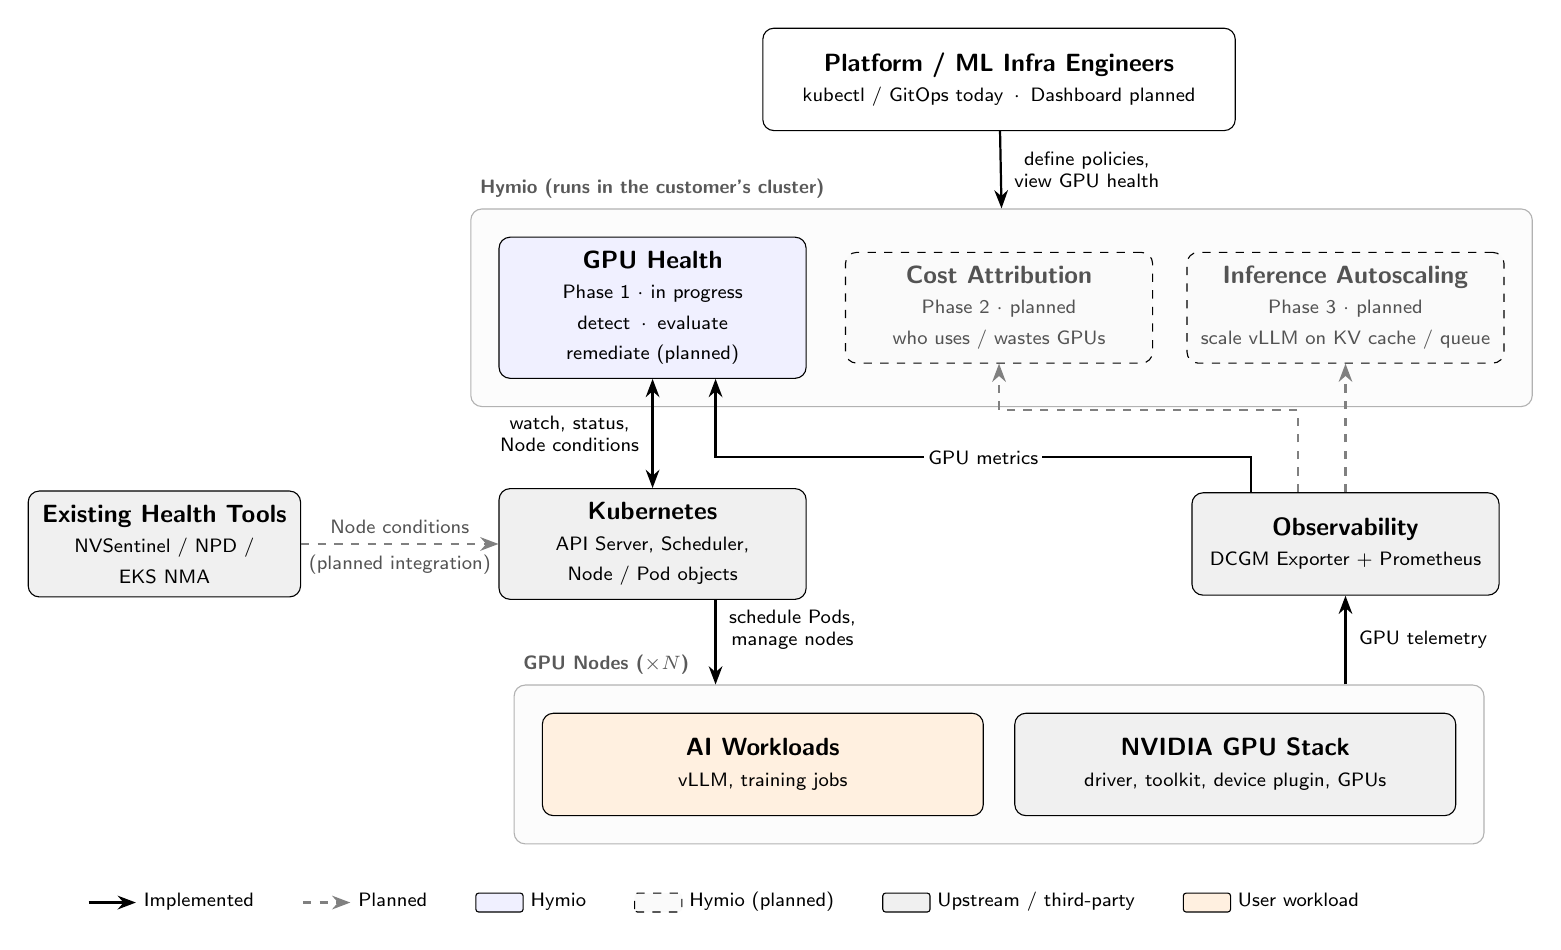
\begin{tikzpicture}[
  font=\sffamily\small,
  base/.style={draw, rounded corners, minimum width=3.9cm, minimum height=1.3cm,
               align=center, inner sep=5pt},
  hymio/.style={base, fill=blue!6},
  upstream/.style={base, fill=gray!12},
  workload/.style={base, fill=orange!12},
  planned/.style={base, dashed, fill=gray!4, text=gray!65!black},
  arrow/.style={-{Stealth}, thick},
  parrow/.style={-{Stealth}, thick, dashed, gray},
  lbl/.style={font=\sffamily\scriptsize, fill=white, inner sep=1.5pt, align=center},
  plbl/.style={lbl, text=gray!65!black},
  group/.style={draw=gray!60, rounded corners, inner sep=10pt, fill=gray!2},
  grouplabel/.style={font=\sffamily\scriptsize\bfseries, text=gray!70!black, anchor=south west}
]

% ---------- Users ----------
\node[base, fill=white, minimum width=6cm] (users) at (0, 0)
  {\textbf{Platform / ML Infra Engineers}\\
   {\scriptsize kubectl / GitOps today \,$\cdot$\, Dashboard planned}};

% ---------- Hymio capabilities ----------
\node[hymio] (health) at (-4.4, -2.9)
  {\textbf{GPU Health}\\{\scriptsize Phase 1 $\cdot$ in progress}\\
   {\scriptsize detect \,$\cdot$\, evaluate}\\{\scriptsize remediate (planned)}};
\node[planned] (cost) at (0, -2.9)
  {\textbf{Cost Attribution}\\{\scriptsize Phase 2 $\cdot$ planned}\\
   {\scriptsize who uses / wastes GPUs}};
\node[planned] (scale) at (4.4, -2.9)
  {\textbf{Inference Autoscaling}\\{\scriptsize Phase 3 $\cdot$ planned}\\
   {\scriptsize scale vLLM on KV cache / queue}};

% ---------- Platform services ----------
\node[upstream] (k8s) at (-4.4, -5.9)
  {\textbf{Kubernetes}\\{\scriptsize API Server, Scheduler,}\\{\scriptsize Node / Pod objects}};
\node[upstream] (obs) at (4.4, -5.9)
  {\textbf{Observability}\\{\scriptsize DCGM Exporter + Prometheus}};
\node[upstream, minimum width=3.4cm] (ext) at (-10.6, -5.9)
  {\textbf{Existing Health Tools}\\{\scriptsize NVSentinel / NPD /}\\{\scriptsize EKS NMA}};

% ---------- GPU nodes ----------
\node[workload, minimum width=5.6cm] (wl) at (-3.0, -8.7)
  {\textbf{AI Workloads}\\{\scriptsize vLLM, training jobs}};
\node[upstream, minimum width=5.6cm] (gpu) at (3.0, -8.7)
  {\textbf{NVIDIA GPU Stack}\\{\scriptsize driver, toolkit, device plugin, GPUs}};

% ---------- Groups ----------
\begin{scope}[on background layer]
  \node[group, fit=(health)(cost)(scale)] (hymiogrp) {};
  \node[grouplabel] at (hymiogrp.north west) {Hymio (runs in the customer's cluster)};
  \node[group, fit=(wl)(gpu)] (nodegrp) {};
  \node[grouplabel] at (nodegrp.north west) {GPU Nodes ($\times N$)};
\end{scope}

% ---------- Arrows ----------
\draw[arrow] (users) -- node[lbl, right=3pt] {define policies,\\view GPU health} (hymiogrp.north);

\draw[arrow, {Stealth}-{Stealth}] (health) -- node[lbl, left=3pt] {watch, status,\\Node conditions} (k8s);
\draw[arrow] ([xshift=-1.2cm]obs.north) |- node[lbl, pos=0.75] {GPU metrics} (-3.6, -4.8) -- (-3.6, -4.8 |- health.south);
\draw[parrow] ([xshift=-0.6cm]obs.north) |- (0, -4.2) -- (cost.south);
\draw[parrow] (obs.north) -- (scale.south);

\draw[arrow] ([xshift=0.8cm]k8s.south) -- node[lbl, pos=0.35, right=3pt] {schedule Pods,\\manage nodes} ([xshift=0.8cm]k8s.south |- nodegrp.north);
\draw[arrow] (obs.south |- nodegrp.north) -- node[lbl, right=3pt] {GPU telemetry} (obs.south);

\draw[parrow] (ext) -- node[plbl, above=2pt, fill=none] {Node conditions} node[plbl, below=2pt, fill=none] {(planned integration)} (k8s);

% ---------- Legend ----------
\node[font=\sffamily\scriptsize, anchor=north west, align=left] at (-11.7, -10.2) {%
  \tikz[baseline=-0.5ex]{\draw[thick,-{Stealth}] (0,0)--(0.6,0);}~Implemented \qquad
  \tikz[baseline=-0.5ex]{\draw[thick,dashed,gray,-{Stealth}] (0,0)--(0.6,0);}~Planned \qquad
  \tikz[baseline=-0.5ex]{\draw[rounded corners=1pt,fill=blue!6] (0,-0.12) rectangle (0.6,0.12);}~Hymio \qquad
  \tikz[baseline=-0.5ex]{\draw[dashed,rounded corners=1pt,fill=gray!4] (0,-0.12) rectangle (0.6,0.12);}~Hymio (planned) \qquad
  \tikz[baseline=-0.5ex]{\draw[rounded corners=1pt,fill=gray!12] (0,-0.12) rectangle (0.6,0.12);}~Upstream / third-party \qquad
  \tikz[baseline=-0.5ex]{\draw[rounded corners=1pt,fill=orange!12] (0,-0.12) rectangle (0.6,0.12);}~User workload
};

\end{tikzpicture}
\end{document}